% 2018.01.08 Modified
% 2015.07.10 Modified
%
% mthesis.tex
%
\documentclass[12pt]{jarticle} % Japanese
%\documentclass[12pt]{article} % English
% if there are problems in the above regarding fonts, use this
% \documentclass[UTF8]{ctexart}

\usepackage[utf8]{inputenc}
%\usepackage{utf}
\usepackage{naist-jmthesis} %Japanese
%\usepackage{naist-mthesis} %English

\usepackage{graphicx}

%
% Page style
%
\pagestyle{final}       % Camera-Ready
%\pagestyle{draft}      % Draft
%
%
\lang{Japanese} % Japanese
%\lang{English} % English
%
% Student Number
%
\studentnumber{1811098}
%
% 修士論文 か 課題研究 かの選択
%
\doctitle{\mastersthesis}       % 修士論文
%\doctitle{\mastersreport}      % 課題研究
%
% 取得予定の修士号は 修士(工学) か 修士(理学) か ?
%
\major{\engineering}    % 工学
%\major{\science}       % 理学
%
% 日本語題目 (in LaTeX)
%
\title{ソースコードの類似性に基づいたテストコード\\自動推薦ツール}
%
% 日本語題目 (in plain text)
%
%   注: (in LaTeX)と同じ場合は指定する必要なし。
%       この情報は修士論文/課題研究には現れませんが、管理のために必要です。
%
\ptitle{太陽と月を利用したpiの低速計算アルゴリズムに関する理論的研究}
%
% 英語題目 (in LaTeX)
%
\etitle{Automatic Test Suite Recommendation System based on Code Clone Detection}
%
% 英語題目 (in plain text)
%
%   注: (in LaTeX)と同じ場合は指定する必要なし。
%       この情報は修士論文/課題研究には現れませんが、管理のために必要です。
%
\eptitle{Theoretical Studies on Low-Speed Calculation Algorithms of pi \\
Utilizing the Sun and the Moon}
%
% 日本語氏名 (in LaTeX)
%   (姓と名の間に空白を入れて下さい)
%
\author{倉地 亮介}
%
% 日本語氏名 (in plain text)
%
%   注: (in LaTeX)と同じ場合は指定する必要なし。
%       この情報は修士論文/課題研究には現れませんが、管理のために必要です。
%
\pauthor{}
%
% 欧文氏名 (in LaTeX)
%   (first name, last name の順に記入し、先頭文字のみを大文字にする。)
%
\eauthor{Ryosuke Kurachi}
% 別の例: \eauthor{Kurt G\"{o}del}
%
%
% 欧文氏名 (in plain text)
%
%   注: (in LaTeX)と同じ場合は指定する必要なし。
%       この情報は修士論文/課題研究には現れませんが、管理のために必要です。
%
\epauthor{}
% 別の例: \peauthor{Kurt Goedel}
%
%
% 論文提出年月日
%
\syear{2020}
\smonth{1}
\sday{28}
%
% 専攻の選択
%
\department{\infproc}  % 情報処理学
%\department{\infsys}    % 情報システム学
%\department{\bioinf}   % 情報生命科学
%\department{\infsci}    % 情報科学
%
%
% 審査委員(日本語)
%   (姓と名、名と称号の間に空白を入れて下さい)
%
%5人以上の場合,5人目以降は\addcmembers を使って宣言する。
%最大で合わせて8人まで宣言可能。
%主指導教員、副指導教員を明記する。両指導教員以外は委員。
%学外審査委員は、大学名を明記する
%
% 4人の場合
\cmembers{飯田 元 教授}{(主指導教員)}
         {井上 美智子 教授}{(副指導教員)}
         {市川 昊平 准教授}{(副指導教員)}
         {崔 恩瀞 准教授}{(京都工芸繊維大学)}
%
% 3人の場合
%\cmembers{○○ ○○ 教授}{(主指導教員)}
%         {○○ ○○ 教授}{(副指導教員)}
%         {○○ ○○ 准教授}{(副指導教員)}
%         {}{}
%
% 2人の場合
%\cmembers{○○ ○○ 教授}{(主指導教員)}
%         {○○ ○○ 教授}{(副指導教員)}
%          {}{}
%          {}{}
%
% 5人目の宣言
%\addcmembers{55 55 准教授}{(□□大学)}
%            {}{}
%            {}{}
%            {}{}
%
% 5〜6人目の宣言
%\addcmembers{55 55 准教授}{(□□大学)}
%            {66 66 准教授}{(□□大学)}
%            {}{}
%            {}{}
%
% 5〜7人目の宣言
%\addcmembers{55 55 准教授}{(□□大学)}
%            {66 66 准教授}{(□□大学)}
%            {77 77 准教授}{(□□大学)}
%            {}{}
%
% 5〜8人目の宣言
%\addcmembers{55 55 准教授}{(□□大学)}
%            {66 66 准教授}{(□□大学)}
%            {77 77 准教授}{(□□大学)}
%            {88 88 准教授}{(□□大学)}
%
%
% 審査委員(英語)
%     (first name, last name の順に記入し、先頭文字のみを大文字にする。
%       first name と last name の間に空白、
%       last name と 称号の間にカンマと空白を入れて下さい。)
%
% 5人以上の場合,5人目以降は\eaddcmembers を使って宣言する
% Supervisor, Co-supervisor, and Member must be specified.
% 4人の場合
\ecmembers{Professor XXX XXX}{(Supervisor)}
          {Professor XXX XXX}{(Co-supervisor)}
          {Associate Professor XXX XXX}{(Co-supervisor)}
          {Associate Professor XXX XXX}{(YY University)}
%
% 3人の場合
%\ecmembers{Professor XXX XXX}{(Supervisor)}
%          {Professor XXX XXX}{(Co-supervisor)}
%          {Associate Professor XXX XXX}{(Co-supervisor)}
%          {}{}
%
% 2人の場合
% \ecmembers{Professor XXX XXX}{(Supervisor)}
%           {Professor XXX XXX}{(Co-supervisor)}
%           {}{}
%           {}{}
%
% 5人目の宣言
%\eaddcmembers{Professor 55 55}{(YY University)}
%            {}{}
%            {}{}
%            {}{}
%
% 5〜6人目の宣言
%\eaddcmembers{Professor 55 55}{(YY University)}
%             {Professor 66 66}{(YY University)}
%             {}{}
%             {}{}
%
% 5〜7人目の宣言
%\eaddcmembers{Professor 55 55}{(YY University)}
%             {Professor 66 66}{(YY University)}
%             {Professor 77 77}{(YY University)}
%             {}{}
%
% 5〜8人目の宣言
%\eaddcmembers{Professor 55 55}{(YY University)}
%             {Professor 66 66}{(YY University)}
%             {Professor 77 77}{(YY University)}
%             {Professor 88 88}{(YY University)}
%
%
%
% キーワード5〜6個 (in LaTeX)
%
\keywords{類似コード検出, 推薦システム, ソフトウェアテスト, 単体テスト}
%
% キーワード5〜6個 (in plain text)
%
%   注: (in LaTeX)と同じ場合は記入する必要なし。
%       この情報は修士論文/課題研究には現れませんが、管理のために必要です。
%
\pkeywords{類似コード検出, 推薦システム, ソフトウェアテスト, 単体テスト}
%
% 5 or 6 Keywords (in LaTeX)
%
\ekeywords{clone detection, recommendation system, software testing, unit test}
%
% 5 or 6 Keywords (in plain text)
%
%   注: (in LaTeX)と同じ場合は記入する必要なし。
%       この情報は修士論文/課題研究には現れませんが、管理のために必要です。
%
\epkeywords{pi, astronomy, mathematics, computer, algorithm}
%
% 内容梗概 (in LaTeX)
%
%   注: 行の先頭が\\で始まらないようにすること。
%
\abstract{
人類がこの地上に現われて以来、$\pi$の計算には多くの関心が払われてきた。

本論文では、太陽と月を利用して$\pi$を低速に計算するための
画期的なアルゴリズムを与える。

ここには内容梗概を書く。ここには内容梗概を書く。ここには内容梗概を書く。
ここには内容梗概を書く。ここには内容梗概を書く。ここには内容梗概を書く。
ここには内容梗概を書く。ここには内容梗概を書く。ここには内容梗概を書く。
ここには内容梗概を書く。ここには内容梗概を書く。ここには内容梗概を書く。
ここには内容梗概を書く。ここには内容梗概を書く。ここには内容梗概を書く。

ここには内容梗概を書く。ここには内容梗概を書く。ここには内容梗概を書く。
ここには内容梗概を書く。ここには内容梗概を書く。ここには内容梗概を書く。
ここには内容梗概を書く。ここには内容梗概を書く。ここには内容梗概を書く。
ここには内容梗概を書く。ここには内容梗概を書く。ここには内容梗概を書く。
ここには内容梗概を書く。ここには内容梗概を書く。ここには内容梗概を書く。
}
%
% 内容梗概 (in plain text)
%
%   注: (in LaTeX)と同じ場合は記入する必要なし。
%       この情報は修士論文/課題研究には現れませんが、管理のために必要です。
%       改行する箇所には空白行を入れる。
%       行の先頭が\\で始まらないようにすること。
%
\pabstract{
人類がこの地上に現われて以来、piの計算には多くの関心が払われてきた。

本論文では、太陽と月を利用してpiを低速に計算するための
画期的なアルゴリズムを与える。

ここには内容梗概を書く。ここには内容梗概を書く。ここには内容梗概を書く。
ここには内容梗概を書く。ここには内容梗概を書く。ここには内容梗概を書く。
ここには内容梗概を書く。ここには内容梗概を書く。ここには内容梗概を書く。
ここには内容梗概を書く。ここには内容梗概を書く。ここには内容梗概を書く。
ここには内容梗概を書く。ここには内容梗概を書く。ここには内容梗概を書く。

ここには内容梗概を書く。ここには内容梗概を書く。ここには内容梗概を書く。
ここには内容梗概を書く。ここには内容梗概を書く。ここには内容梗概を書く。
ここには内容梗概を書く。ここには内容梗概を書く。ここには内容梗概を書く。
ここには内容梗概を書く。ここには内容梗概を書く。ここには内容梗概を書く。
ここには内容梗概を書く。ここには内容梗概を書く。ここには内容梗概を書く。
}
%
% Abstract (in LaTeX)
%
%  注:  行の先頭が\\で始まらないようにすること。
%
\eabstract{
Automatically generated tests tend to be less read-able and maintainable since they often do not consider thelatent objective of the target code. Reusing existing tests mighthelp address this problem. To this end, we present SuiteRec, asystem that recommends reusable test suites based on code clonedetection. Given a java method, SuiteRec searches for its codeclones from a code base collected from open-source projects,and then recommends test suites of the clones. It also providesthe ranking of the recommended test suites computed basedon the similarity between the input code and the cloned code.We evaluate SuiteRec with a human study of ten students. Theresults indicate that SuiteRec successfully recommends reusabletest suites.
}
%
% Abstract (in plain text)
%
%   注: (in LaTeX)と同じ場合は記入する必要なし。
%       この情報は修士論文/課題研究には現れませんが、管理のために必要です。
%       改行する箇所には空白行を入れる。
%       行の先頭が\\で始まらないようにすること。
%
\epabstract{
The calculation of pi has been paid much attention since human beings
appeared on the earth.

This thesis presents novel low-speed algorithms to calculate
pi utilizing the sun and the moon.

This is a sample abstract. This is a sample abstract. 
This is a sample abstract. This is a sample abstract. 
This is a sample abstract. This is a sample abstract. 
This is a sample abstract. This is a sample abstract. 
This is a sample abstract. This is a sample abstract. 

This is a sample abstract. This is a sample abstract. 
This is a sample abstract. This is a sample abstract. 
This is a sample abstract. This is a sample abstract. 
This is a sample abstract. This is a sample abstract. 

}
%%%%%%%%%%%%%%%%%%%%%%%%% document starts here %%%%%%%%%%%%%%%%%%%%%%%%%%%%
\begin{document}
%
% 表紙 および アブストラクト
%
\titlepage
\cmemberspage
\firstabstract
\secondabstract
%
% 目次
%
\toc
\newpage
\listoffigures
%\newpage
\listoftables
%
% これ以降本文
%
\newpage
\section{はじめに}
\pagenumbering{arabic}

はじめに はじめに はじめに はじめに はじめに はじめに はじめに はじめに 
はじめに はじめに はじめに はじめに はじめに はじめに はじめに はじめに 
はじめに はじめに はじめに はじめに はじめに はじめに はじめに はじめに 

はじめに はじめに はじめに はじめに はじめに はじめに はじめに はじめに 
はじめに はじめに はじめに はじめに はじめに はじめに はじめに はじめに 
はじめに はじめに はじめに はじめに はじめに はじめに はじめに はじめに 

\ref{kako}節では、過去における研究について述べ、
\ref{kadai}章では、現状と今後の課題について述べる。
また、付録\ref{omake1}におまけその1を添付する。


\subsection{過去における研究}
\label{kako}


\begin{figure*}[t]
 \centering
% 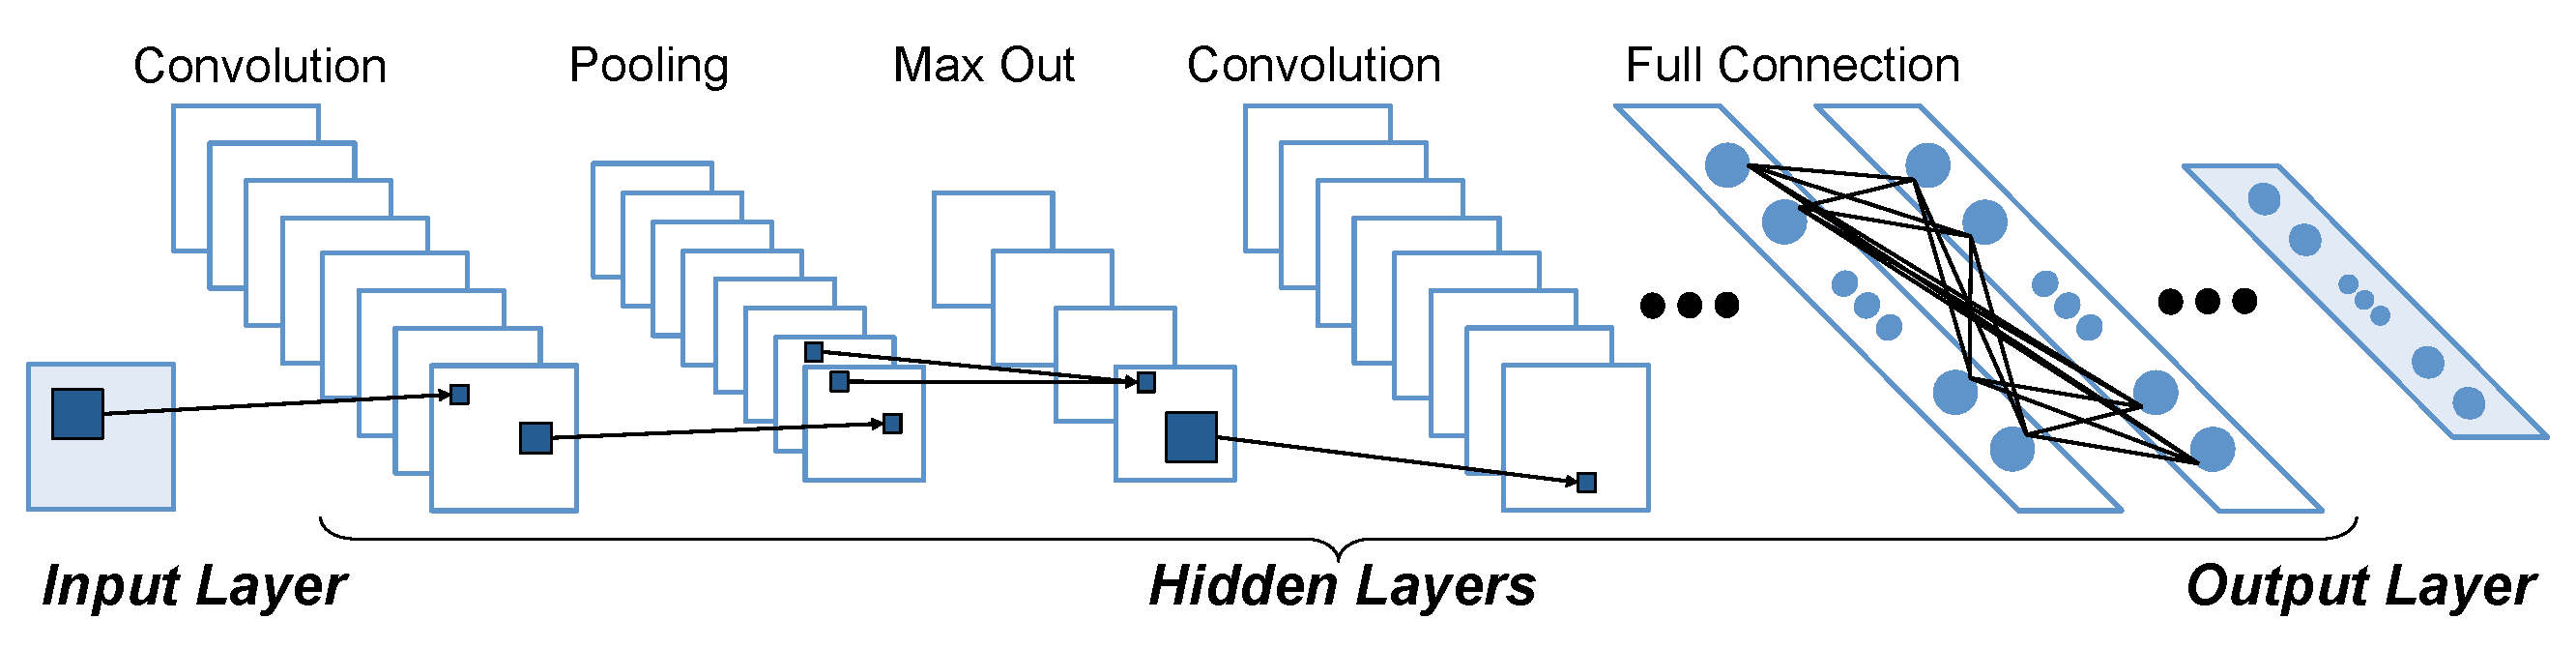
\includegraphics[width=0.8\textwidth,keepaspectratio,clip]{fig/cnn.eps}
 \caption{Convolutional Neural Network (CNN)}
 \label{fig:CNN}
\end{figure*}

過去における研究としては\cite{alex_nips12}などがある。

過去における研究 過去における研究 過去における研究 
過去における研究 過去における研究 過去における研究 過去における研究 
過去における研究 過去における研究 過去における研究 過去における研究 

過去における研究 過去における研究 過去における研究 過去における研究 
過去における研究 過去における研究 過去における研究 過去における研究 
過去における研究 過去における研究 過去における研究 過去における研究 
過去における研究 過去における研究 過去における研究 過去における研究 
過去における研究 過去における研究 過去における研究 過去における研究 

過去における研究 過去における研究 過去における研究 過去における研究 
過去における研究 過去における研究 過去における研究 過去における研究 
過去における研究 過去における研究 過去における研究 過去における研究 
過去における研究 過去における研究 過去における研究 過去における研究 
過去における研究 過去における研究 過去における研究 過去における研究 

\subsection{研究の目的と意義}

研究の目的と意義 研究の目的と意義 研究の目的と意義 研究の目的と意義 
研究の目的と意義 研究の目的と意義 研究の目的と意義 研究の目的と意義 
研究の目的と意義 研究の目的と意義 研究の目的と意義 研究の目的と意義 
研究の目的と意義 研究の目的と意義 研究の目的と意義 研究の目的と意義 

研究の目的と意義 研究の目的と意義 研究の目的と意義 研究の目的と意義 
研究の目的と意義 研究の目的と意義 研究の目的と意義 研究の目的と意義 
研究の目的と意義 研究の目的と意義 研究の目的と意義 研究の目的と意義 
研究の目的と意義 研究の目的と意義 研究の目的と意義 研究の目的と意義 

研究の目的と意義 研究の目的と意義 研究の目的と意義 研究の目的と意義 
研究の目的と意義 研究の目的と意義 研究の目的と意義 研究の目的と意義 
研究の目的と意義 研究の目的と意義 研究の目的と意義 研究の目的と意義 
研究の目的と意義 研究の目的と意義 研究の目的と意義 研究の目的と意義 

\begin{figure}
\centerline{ここに図を書く}
\caption{これは図の例}
\end{figure}

\begin{table}
\centerline{ここに表を書く}
\caption{これは表の例}
\end{table}

研究の目的と意義 研究の目的と意義 研究の目的と意義 研究の目的と意義 
研究の目的と意義 研究の目的と意義 研究の目的と意義 研究の目的と意義 
研究の目的と意義 研究の目的と意義 研究の目的と意義 研究の目的と意義 
研究の目的と意義 研究の目的と意義 研究の目的と意義 研究の目的と意義 

研究の目的と意義 研究の目的と意義 研究の目的と意義 研究の目的と意義 
研究の目的と意義 研究の目的と意義 研究の目的と意義 研究の目的と意義 
研究の目的と意義 研究の目的と意義 研究の目的と意義 研究の目的と意義 
研究の目的と意義 研究の目的と意義 研究の目的と意義 研究の目的と意義 

研究の目的と意義 研究の目的と意義 研究の目的と意義 研究の目的と意義 
研究の目的と意義 研究の目的と意義 研究の目的と意義 研究の目的と意義 
研究の目的と意義 研究の目的と意義 研究の目的と意義 研究の目的と意義 
研究の目的と意義 研究の目的と意義 研究の目的と意義 研究の目的と意義 

研究の目的と意義 研究の目的と意義 研究の目的と意義 研究の目的と意義 
研究の目的と意義 研究の目的と意義 研究の目的と意義 研究の目的と意義 
研究の目的と意義 研究の目的と意義 研究の目的と意義 研究の目的と意義 
研究の目的と意義 研究の目的と意義 研究の目的と意義 研究の目的と意義 

研究の目的と意義 研究の目的と意義 研究の目的と意義 研究の目的と意義 
研究の目的と意義 研究の目的と意義 研究の目的と意義 研究の目的と意義 
研究の目的と意義 研究の目的と意義 研究の目的と意義 研究の目的と意義 
研究の目的と意義 研究の目的と意義 研究の目的と意義 研究の目的と意義 

研究の目的と意義 研究の目的と意義 研究の目的と意義 研究の目的と意義 
研究の目的と意義 研究の目的と意義 研究の目的と意義 研究の目的と意義 
研究の目的と意義 研究の目的と意義 研究の目的と意義 研究の目的と意義 
研究の目的と意義 研究の目的と意義 研究の目的と意義 研究の目的と意義 

研究の目的と意義 研究の目的と意義 研究の目的と意義 研究の目的と意義 
研究の目的と意義 研究の目的と意義 研究の目的と意義 研究の目的と意義 
研究の目的と意義 研究の目的と意義 研究の目的と意義 研究の目的と意義 
研究の目的と意義 研究の目的と意義 研究の目的と意義 研究の目的と意義 

研究の目的と意義 研究の目的と意義 研究の目的と意義 研究の目的と意義 
研究の目的と意義 研究の目的と意義 研究の目的と意義 研究の目的と意義 
研究の目的と意義 研究の目的と意義 研究の目的と意義 研究の目的と意義 
研究の目的と意義 研究の目的と意義 研究の目的と意義 研究の目的と意義 

研究の目的と意義 研究の目的と意義 研究の目的と意義 研究の目的と意義 
研究の目的と意義 研究の目的と意義 研究の目的と意義 研究の目的と意義 
研究の目的と意義 研究の目的と意義 研究の目的と意義 研究の目的と意義 
研究の目的と意義 研究の目的と意義 研究の目的と意義 研究の目的と意義 

研究の目的と意義研究の目的と意義研究の目的と意義研究の目的と意義 
研究の目的と意義研究の目的と意義研究の目的と意義研究の目的と意義 
研究の目的と意義研究の目的と意義研究の目的と意義研究の目的と意義 
研究の目的と意義研究の目的と意義研究の目的と意義研究の目的と意義 

研究の目的と意義研究の目的と意義研究の目的と意義研究の目的と意義 
研究の目的と意義研究の目的と意義研究の目的と意義研究の目的と意義 
研究の目的と意義研究の目的と意義研究の目的と意義研究の目的と意義 
研究の目的と意義研究の目的と意義研究の目的と意義研究の目的と意義 

研究の目的と意義研究の目的と意義研究の目的と意義研究の目的と意義 
研究の目的と意義研究の目的と意義研究の目的と意義研究の目的と意義 
研究の目的と意義研究の目的と意義研究の目的と意義研究の目的と意義 
研究の目的と意義研究の目的と意義研究の目的と意義研究の目的と意義 


\newpage

This page is written in English. This page is written in English. 
This page is written in English. This page is written in English. 
This page is written in English. This page is written in English. 
This page is written in English. This page is written in English. 

This page is written in English. This page is written in English. 
This page is written in English. This page is written in English. 
This page is written in English. This page is written in English. 
This page is written in English. This page is written in English. 

This page is written in English. This page is written in English. 
This page is written in English. This page is written in English. 
This page is written in English. This page is written in English. 
This page is written in English. This page is written in English. 

This page is written in English. This page is written in English. 
This page is written in English. This page is written in English. 
This page is written in English. This page is written in English. 
This page is written in English. This page is written in English. 

This page is written in English. This page is written in English. 
This page is written in English. This page is written in English. 
This page is written in English. This page is written in English. 
This page is written in English. This page is written in English. 

This page is written in English. This page is written in English. 
This page is written in English. This page is written in English. 
This page is written in English. This page is written in English. 
This page is written in English. This page is written in English. 

This page is written in English. This page is written in English. 
This page is written in English. This page is written in English. 
This page is written in English. This page is written in English. 
This page is written in English. This page is written in English. 
This page is written in English. This page is written in English. 
This page is written in English. This page is written in English. 
This page is written in English. This page is written in English. 
This page is written in English. This page is written in English. 

This page is written in English. This page is written in English. 
This page is written in English. This page is written in English. 
This page is written in English. This page is written in English. 
This page is written in English. This page is written in English. 
This page is written in English. This page is written in English. 
This page is written in English. This page is written in English. 
This page is written in English. This page is written in English. 
This page is written in English. This page is written in English. 

This page is written in English. This page is written in English. 
This page is written in English. This page is written in English. 
This page is written in English. This page is written in English. 
This page is written in English. This page is written in English. 
This page is written in English. This page is written in English. 
This page is written in English. This page is written in English. 
This page is written in English. This page is written in English. 
This page is written in English. This page is written in English. 


\newpage
\section{現状と今後の課題}
\label{kadai}

現状と今後の課題 現状と今後の課題 現状と今後の課題 現状と今後の課題 
現状と今後の課題 現状と今後の課題 現状と今後の課題 現状と今後の課題 
現状と今後の課題 現状と今後の課題 現状と今後の課題 現状と今後の課題 
現状と今後の課題 現状と今後の課題 現状と今後の課題 現状と今後の課題 

現状と今後の課題 現状と今後の課題 現状と今後の課題 現状と今後の課題 
現状と今後の課題 現状と今後の課題 現状と今後の課題 現状と今後の課題 
現状と今後の課題 現状と今後の課題 現状と今後の課題 現状と今後の課題 
現状と今後の課題 現状と今後の課題 現状と今後の課題 現状と今後の課題 

現状と今後の課題 現状と今後の課題 現状と今後の課題 現状と今後の課題 
現状と今後の課題 現状と今後の課題 現状と今後の課題 現状と今後の課題 
現状と今後の課題 現状と今後の課題 現状と今後の課題 現状と今後の課題 
現状と今後の課題 現状と今後の課題 現状と今後の課題 現状と今後の課題 

%
% 謝辞
%
\acknowledgements

Thank you. Thank you.
%
% 参考文献
% ここでは \reference を使って、自分でリストを作るか、BibTeX を使って
% リストをつくって下さい。この例では BibTeX を作るような形式になってい
% ます。
%
\newpage
% \reference
\bibliographystyle{plain}
\bibliography{mthesis}
%
% 付録
%
\appendix

\section{おまけその1}
\label{omake1}

これはおまけです。これはおまけです。これはおまけです。これはおまけです。
これはおまけです。これはおまけです。これはおまけです。これはおまけです。
これはおまけです。これはおまけです。これはおまけです。これはおまけです。
これはおまけです。これはおまけです。これはおまけです。これはおまけです。

\begin{figure}
\centerline{これはおまけの図です。}
\caption{おまけの図}
\end{figure}


\section{おまけその2}

これもおまけです。これもおまけです。これもおまけです。これもおまけです。
これもおまけです。これもおまけです。これもおまけです。これもおまけです。
これもおまけです。これもおまけです。これもおまけです。これもおまけです。
これもおまけです。これもおまけです。これもおまけです。これもおまけです。

\end{document}

